\documentclass{article}
\usepackage[utf8]{inputenc}  % Para caracteres acentuados
\usepackage{booktabs}        % Para \toprule, \midrule, \bottomrule
\usepackage{graphicx}        % Para inserir figuras
\usepackage{float}           % Para usar [H] e fixar posição da figura
\usepackage{lipsum}          % Para texto de exemplo (opcional)

\begin{document}
	
	% --- Espaço para texto introdutório ---
	
	

	% --- Gráfico centralizado template---
	\section*{Gráfico}
	\begin{figure}[H]
		\centering
		\caption{Boxplot dos resultados de 36 exames de sangue, referente à fração de colesterol de muito baixa
			densidade (VLDL), em miligramas por decilitro (mg/dL), em indivíduos do sexo feminino.}
		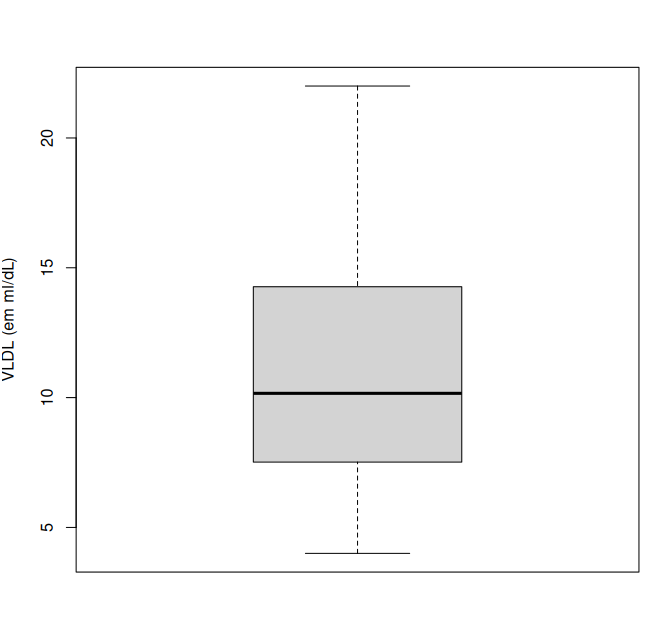
\includegraphics[width=0.7\textwidth]{/home/thallysson/Área de trabalho/Disciplinas/Estatistica/latex/graficos/grafico_atv4.png} % substitua pelo arquivo do seu gráfico
		
		\label{fig:grafico_filhos}
	\end{figure}
	
	% --- Espaço para análise ou comentários ---
	\section*{Análise}
	De acordo com a figura 1, os dados não possuem outliers, e sua distribuição de frequência é assimétrica a direita, o que significa que sua moda é menor que a mediana, e a mediana é menor que a média. O intervalo entre os quartis com a menor variância são os valoers entre o primeiro aqurtil e a mediana. Já o intervalo com a maior variância são os valores entre o terceiro quartil e o maior valor.
	
	
\end{document}

